%TeX

\documentclass{beamer}

\usepackage{graphicx}
\graphicspath{ {include/images/} }
\usepackage{verbatim}
\usepackage{xspace}
\usepackage{tikz}

% just for the vaporsec text
\usepackage{xeCJK}

% \usetheme{DarkConsole}
\usetheme{Madrid}
\useinnertheme{rectangles}
\setbeamercolor{normal text}{bg=black!05}

\newcommand{\VaporSec}{
    \symbol{65334}\symbol{65313}\symbol{65328}\symbol{65327}\symbol{65330}%
    \symbol{65331}\symbol{65317}\symbol{65315}
}

\newcommand{\Aesthetic}{
    \symbol{65313}\symbol{65317}\symbol{65331}\symbol{65332}\symbol{65320}%
    \symbol{65317}\symbol{65332}\symbol{65321}\symbol{65315}
}

\newcommand{\Aesthetics}{\Aesthetic\symbol{65331}}

\title{For Realz Mode!}
\subtitle{
    Reversing an MBR from the CSAW CTF\\
    {\em (and how to write a keygen with a SAT solver)}
}
\author{@t0x0 \and @numinit}
\institute{\VaporSec}
\date{2017-XX-YY}

\begin{document}
\begin{frame}
    \titlepage
\end{frame}

%TeX

\section{Introduction}

\begin{frame}{About us}
    \begin{itemize}
        \item Morgan (@numinit)
        \begin{itemize}
            \item Software developer by day
            \item Tinkerer on everything by night
            \item First Def Con and Toorcon experiences this year
            \item Doing CSAW CTF for a while
        \end{itemize}
        \item t0x0 (@t0x0pg)
        \begin{itemize}
            \item Writes lots of interpreted code
            \item Lives mostly in Windows world
            \item Jack of all trades, master of none (so far)
            \item Obsessively curious
        \end{itemize}
    \end{itemize}
\end{frame}

\begin{frame}{What's CSAW?}
    \begin{columns}
        \column{0.5\textwidth}
        An annual security capture the flag run by New York Polytechnic that
        contains challenges with a \alert{wide range of difficulties},
        attracting everyone from undergraduates to well-known teams

        \column{0.5\textwidth}
        \Graphic{csaw-logo} \\
        \Graphic{scoreboard}
    \end{columns}
\end{frame}

\begin{frame}{What's a security capture the flag?}
    \begin{itemize}
        \item<1-> 48 hours of caffeinated reverse engineering and exploitation
        \item<2-> More seriously: an event where you break a bunch of programs
                  to retrieve hidden strings of text (the flags)
        \item<3-> An opportunity to learn new things - we wouldn't
                  even be presenting if it wasn't for this CTF
    \end{itemize}
\end{frame}

\begin{frame}{Who are \VaporSec?}
    \begin{itemize}
        \item A new \Aesthetic San Diego CTF team
        \item Had 10 participants during the CSAW CTF
        \item Achieved 15th in CSAW industry professional bracket, not bad for
              the first time
    \end{itemize}
\end{frame}

%TeX

\section{Reversing the MBR}

\begin{frame}{RE400 what?\ldots}
    \begin{columns}
        \column{0.5\textwidth}
	        \begin{itemize}
                \item Challenge worth 400 points
                \item Reverse Engineering category
                \item We get some hints right away\ldots
                \begin{itemize}
                	\item This is an MBR
                	\item \ldots from an x86 system
        	    \end{itemize}
            \end{itemize}
        \column{0.5\textwidth}
                {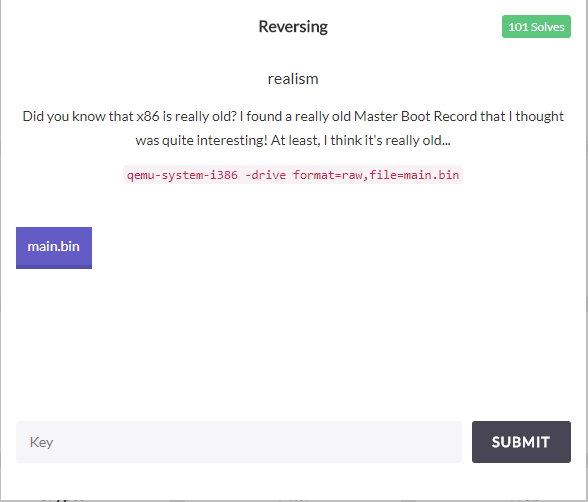
\includegraphics[width=\textwidth]{re400}}
    \end{columns}
\end{frame}

\begin{frame}{A place to start\ldots}
    \begin{columns}
        \column{0.5\textwidth}
	        \begin{itemize}
                \item<1-> Wikipedia, of course!
		        \begin{itemize}
    	            \item<2-> 512 bytes
        	        \item<2-> MBR signature: 55 AA
            	    \item<2-> "expected to contain real mode machine language instructions"
                	\item<2-> little-endian
                	\item<2-> loads at 0000:7C00
	            \end{itemize}                	
            \end{itemize}
        \column{0.5\textwidth}
                {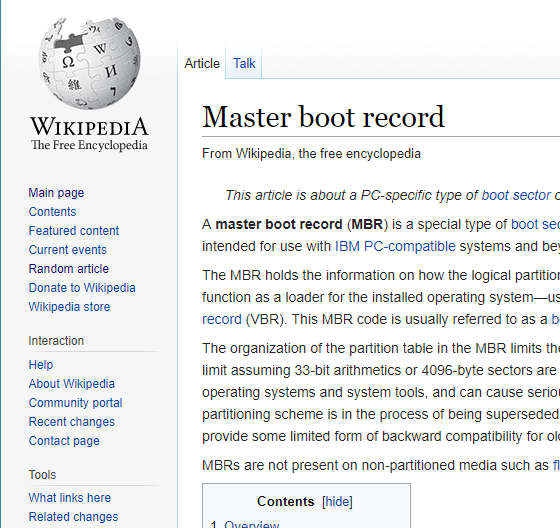
\includegraphics[width=\textwidth]{wikimbr}}
    \end{columns}
\end{frame}

\begin{frame}{Tool Time!\ldots}
    \framesubtitle{qemu (gift wrapped)}
    \begin{columns}
        \column{0.5\textwidth}
            \only<1> {
              	\begin{itemize}
             		\item -s (gdb)
                	\item -S (suspend)
        	       	\item -vnc:1
	            \end{itemize}
            }
            \only<2> {
             	\begin{itemize}
            		\item QEMU/Monitor
              		\begin{itemize}
	    	        	\item info registers
    	    	       	\item system reset
    	    	    \end{itemize}
        	    \end{itemize}
        	}
        \column{0.5\textwidth}
            \only<1>{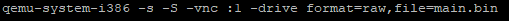
\includegraphics[width=\textwidth]{launch-qemu}\newline\newline
            		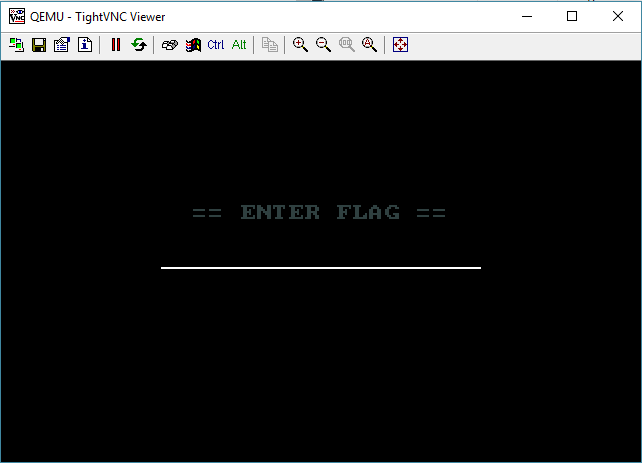
\includegraphics[width=\textwidth]{qemu-vnc}
			}
            \only<2>{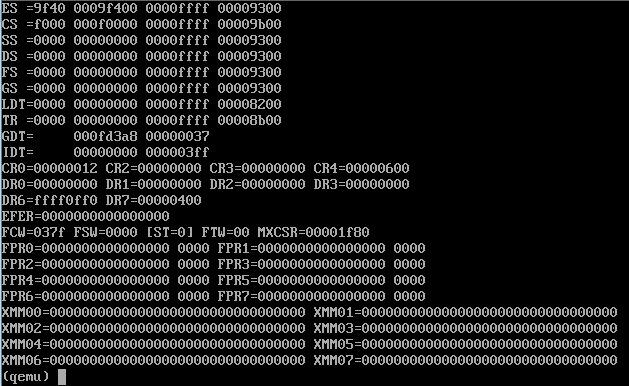
\includegraphics[width=\textwidth]{qemu-info-registers-1}}
    \end{columns}
\end{frame}

\begin{frame}{Tool Time!\ldots}
    \framesubtitle{gdb}
    \begin{columns}
        \column{0.5\textwidth}
                \begin{itemize}
                	\only<1>{
						\item target remote localhost:1234
						\item set architecture i8086
							(bootloaders are 16 bit, right?)
						\item display/i \$pc - print program counter
						\item br *0xADDR - set breakpoint
						\item si - run one instruction
						\item c - continue
					}
					\only<2->{
						\item info reg
						\uncover<3->{\item info frame}
						\uncover<4->{\item x /CT 0xADDR - display C units of T type from ADDR
									\item set {int}0xADDR = 42
									\item set {char[4]} 0xADDR = "AAA"
						}
					}
				\end{itemize}
		\column{0.5\textwidth}
				\only<1>{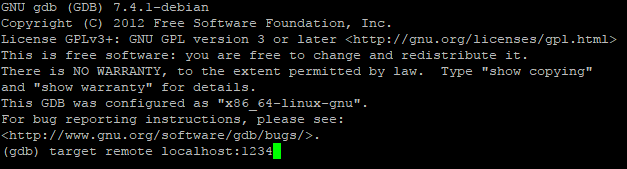
\includegraphics[width=\textwidth]{launch-gdb}\newline\newline
						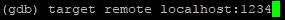
\includegraphics[width=\textwidth]{gdb-target}}
				\only<2>{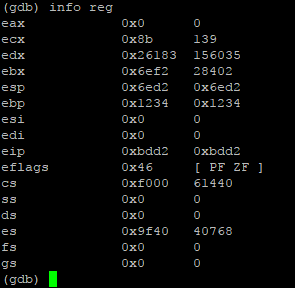
\includegraphics[width=\textwidth]{gdb-info-reg-1}}
				\only<3>{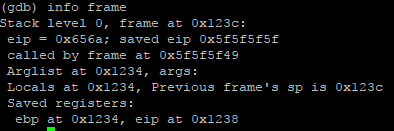
\includegraphics[width=\textwidth]{gdb-info-frame}}
				\only<4-5>{
					\uncover<4->{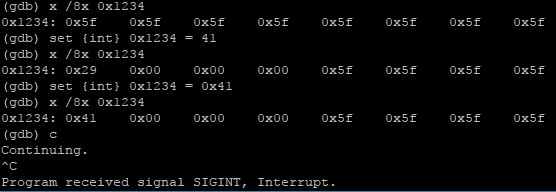
\includegraphics[width=\textwidth]{gdb-x-set-1}}
					\uncover<5->{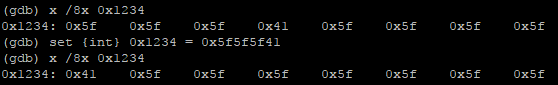
\includegraphics[width=\textwidth]{gdb-x-set-2}}
				}
				\only<6>{
					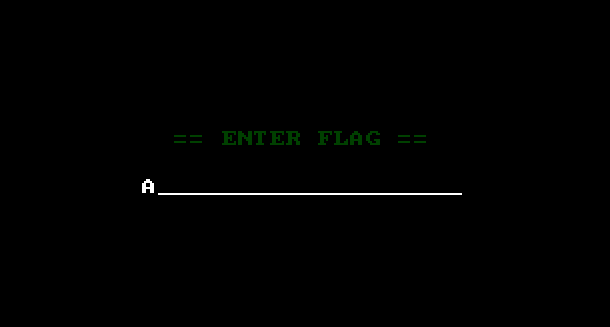
\includegraphics[width=\textwidth]{after-set}
				}
	\end{columns}
\end{frame}
%TeX

\section{Finding the flag}

\begin{frame}{A quick recap\ldots}
    \begin{columns}
        \column{0.5\textwidth}
        \begin{itemize}
            \item<1-> We have an x86 boot sector that's asking us for the flag
            \item<2-> The flag is clearly in the boot sector SOMEWHERE\ldots
            \begin{itemize}
                \item<3-> \ldots but not in plaintext, because this is a 400
                          point challenge and that would be too easy
            \end{itemize}
            \item<4-> So, where is it?
        \end{itemize}
        \column{0.5\textwidth}
        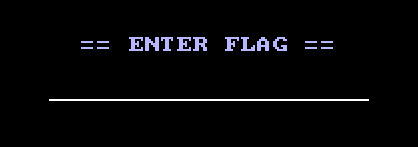
\includegraphics[width=\textwidth]{enter-flag}
    \end{columns}
\end{frame}

\begin{frame}{Reversing the boot sector}
    \begin{columns}
        \column{0.5\textwidth}
        \begin{itemize}
            \item<1-> Open the file in your favorite disassembler (e.g. IDA);
                      rebase at \texttt{0x7c00}
            \item<2-> We can visally pick out three sections:
            \begin{itemize}
                \item<2-> Init code (responsible for the protected
                          mode transition)
                \item<2-> Display code (identifiable by a large number of
                          \texttt{int} instructions)
                \item<2-> Some other code that uses Intel SSE2 instructions
            \end{itemize}
        \end{itemize}
        \column{0.5\textwidth}
        \begin{tikzpicture}
            \only<1> {\node (cfg) {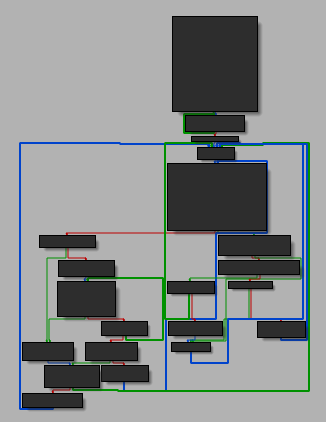
\includegraphics[width=\textwidth]{cfg}};}
            \uncover<2-> {\node (cfga) 
                {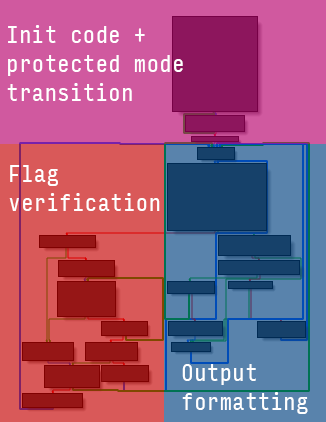
\includegraphics[width=\textwidth]{cfg-annotated}};}
        \end{tikzpicture}
    \end{columns}
\end{frame}

\begin{frame}{First leads}
    \begin{itemize}
        \item<1-> The program asks you to enter 20 characters, and immediately
                  breaks out if the first 4 characters aren't 'flag' after you
                  enter character \#20
        \item<2-> We can verify this in a debugger after eyeballing the code

        \begin{center}
            \uncover<3-> {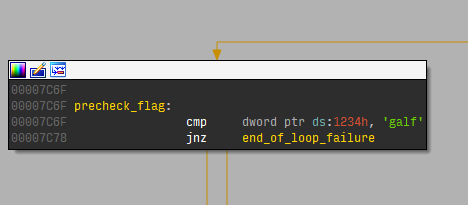
\includegraphics[width=0.7\textwidth]{flag-precheck}}
        \end{center}
    \end{itemize}
\end{frame}

\begin{frame}{As it turns out\ldots}
    \framesubtitle{After several hours of staring at x86 assembly}

    \begin{itemize}
        \item<1-> The flag is \alert{hashed} using a \alert{custom algorithm}
                  implemented with Intel SSE instructions
        \item<2-> {\em Ugh\ldots}
        \item<3-> We have to find an input to the hash algorithm that hashes
                  to the same value stored in the boot sector
    \end{itemize}
\end{frame}

\begin{frame}{Suddenly, SSE2 instructions}
    \framesubtitle{``My Intel CPU can do {\em that?}''}
    The author of the challenge decided to use a bunch of obscure x86 SSE2
    instructions to force us to trawl through Intel documentation

    \begin{itemize}
        \item<2-> movaps\uncover<3->{: Moves to/from/between XMM registers}
        \item<2-> \alert<4->{andps}\uncover<3->{: Performs bitwise AND between
                                                XMM registers}
        \item<2-> pshufd\uncover<3->{: Reorders 32-bit words in XMM registers}
        \item<2-> \alert<4->{psadbw}\uncover<3->{: Sums absolute values of
                                                 differences between bytes
                                                 (it's as crazy as it sounds)}
    \end{itemize}

    \begin{block}<1->{Note}
        SSE2 instructions operate on XMM registers, which are 128 bits
        (16 bytes) wide.
    \end{block}

    \begin{alertblock}<4>{Question}
        Why are these instructions useful for writing a hash function (even if
        it's a bad hash function that we can break?)
    \end{alertblock}
\end{frame}

\newcommand{\StartCell}[2]{
    \node at (0,0) (#1) {\texttt{#2}};%
}
\newcommand{\Cell}[3]{
    \node [anchor=west] at (#1.east) (#2) {\texttt{#3}};%
}

\newcommand{\Xmm}[2]{%
    \getargsC{#2}%
    \raisebox{0.5em}{\texttt{xmm#1}:\xspace}%
    \begin{tikzpicture}[%
        every node/.style={%
            minimum width=1.5em,
            minimum height=0.75em,
            text height=0.75em,
            text depth=0.25em,
            outer sep=0pt,
            draw=black,
            semithick
        }
    ]%
        \StartCell{A}{\argi}%
        \Cell{A}{B}{\argii}%
        \Cell{B}{C}{\argiii}%
        \Cell{C}{D}{\argiv}%
        \Cell{D}{E}{\argv}%
        \Cell{E}{F}{\argvi}%
        \Cell{F}{G}{\argvii}%
        \Cell{G}{H}{\argviii}%
        \Cell{H}{I}{\argix}%
        \Cell{I}{J}{\argx}%
        \Cell{J}{K}{\argxi}%
        \Cell{K}{L}{\argxii}%
        \Cell{L}{M}{\argxiii}%
        \Cell{M}{N}{\argxiv}%
        \Cell{N}{O}{\argxv}%
        \Cell{O}{P}{\argxvi}%
    \end{tikzpicture}%
}

\newcommand{\Left}[1]{\textcolor<5->{red}{#1}}

\newcommand{\Right}[1]{\textcolor<5->{orange}{#1}}

\begin{frame}{Packed Sum of Absolute Differences of Bytes in Word}
    \framesubtitle{That's a mouthful\ldots}
    \begin{center}
        \Xmm{0}{0 1 2 3 4 5 6 7 8 9 10 11 12 13 14 15} \pause \\
        \raisebox{0.3em}{\scriptsize\em (minus)} \\
        \Xmm{1}{15 14 13 12 11 10 9 8 7 6 5 4 3 2 1 0} \pause \\
        \raisebox{0.3em}{\scriptsize $\downarrow$} \\
        \Xmm{0}{-15 -13 -11 -9 -7 -5 -3 -1 1 3 5 7 9 11 13 15} \pause \\
        \raisebox{0.3em}{\scriptsize\em (absolute values)} \\
        \Xmm{0}{%
            \Left{15}
            \Left{13}
            \Left{11}
            \Left{9}
            \Left{7}
            \Left{5}
            \Left{3}
            \Left{1}
            \Right{1}
            \Right{3}
            \Right{5}
            \Right{7}
            \Right{9}
            \Right{11}
            \Right{13}
            \Right{15}
        } \pause \\
        \raisebox{0.3em}{\scriptsize\em (16-bit sums)} \\
        \Xmm{0}{%
            0 0 0 0 0 0 \Left{64} \Left{0} 0 0 0 0 0 0 \Right{64} \Right{0}
        } \\
        \pause
        \begin{alertblock}{It's hard to go back\ldots}
            If you just have the result, you have to find two sets of eight
            bytes where the absolute values of their differences sum to 64
            (and there are many)
        \end{alertblock}
    \end{center}
\end{frame}

\newcounter{SudokuRowCount}
\newcounter{SudokuColCount}
\newcounter{SudokuColIndex}
\newcommand{\SudokuRow}[1]{%
    \setcounter{SudokuColIndex}{0}%
    \setcounter{SudokuColCount}{1}%
    \getargsC{#1}%
    \whiledo{\value{SudokuColIndex} < \narg}{%
        \pgfmathparse{\value{SudokuColCount} - 0.5}%
        \edef\x{\pgfmathresult}%
        \pgfmathparse{\SudokuSize + 0.5 - \value{SudokuRowCount}}%
        \edef\y{\pgfmathresult}%
        \stepcounter{SudokuColIndex}%
        \edef\n{\csname arg\roman{SudokuColIndex}\endcsname}%
        \node[anchor=center] at (\x, \y) {\texttt{\n}};%
        \stepcounter{SudokuColCount}%
    }%
    \stepcounter{SudokuRowCount}%
}

\NewEnviron{sudoku}[2]{%
    \begin{tikzpicture}[
        scale=#2,
        every node/.style={%
            text depth=-0.75ex,
            text height=0.5ex
        }
    ]%
        \pgfmathsetmacro{\SudokuSize}{pow(#1, 2)}%
        \draw (0, 0) grid (\SudokuSize, \SudokuSize);%
        \draw[very thick, scale=#1] (0, 0) grid (#1, #1);%
        \setcounter{SudokuRowCount}{1}%
        \BODY
    \end{tikzpicture}%
}

\begin{frame}{SAT solvers to the rescue!}
    \framesubtitle{How to master Sudoku without memorizing strategies}
    \begin{columns}
        \column{0.5\textwidth}
        {\em
            ``I think a serious case can be made that the decline in the
            American economy can be blamed on the sapping of the mental energy
            and productivity of the American workforce that sudoku addiction
            alone has wrought''
        } \\
        \begin{flushright}
            -- Some Slate writer \\
        \end{flushright}

        \pause 
        Notice anything strange about this puzzle?
        \column{0.5\textwidth}
        \begin{sudoku}{4}{0.33}
            \SudokuRow{\alert<3->{d} \alert<3->{c} \alert<3->{6} \alert<3->{1} \alert<3->{9} 0 e b 5 7 3 2 4 8 f a}
            \SudokuRow{5 8 a 4 f c 2 d 9 0 b e 3 7 6 1}
            \SudokuRow{2 b 9 7 5 3 6 1 4 8 a f d 0 e c}
            \SudokuRow{0 3 f e 4 a 8 7 \alert<3->{d} \alert<3->{c} \alert<3->{6} \alert<3->{1} \alert<3->{9} b 2 5}
            \SudokuRow{8 \alert<3->{d} \alert<3->{c} \alert<3->{6} \alert<3->{1} \alert<3->{9} 3 2 b 5 e 7 0 4 a f}
            \SudokuRow{b 1 5 0 d 8 c 6 f a 9 4 7 2 3 e}
            \SudokuRow{9 a 4 f 7 5 0 e 2 3 1 8 b d c 6}
            \SudokuRow{7 2 e 3 b 4 a f 0 \alert<3->{d} \alert<3->{c} \alert<3->{6} \alert<3->{1} \alert<3->{9} 5 8}
            \SudokuRow{e 4 \alert<3->{d} \alert<3->{c} \alert<3->{6} \alert<3->{1} \alert<3->{9} 0 a b 2 5 8 f 7 3}
            \SudokuRow{1 9 8 2 3 7 5 4 e 6 f 0 a c d b}
            \SudokuRow{f 6 7 a 2 d b c 1 9 8 3 5 e 0 4}
            \SudokuRow{3 5 0 b a e f 8 7 4 \alert<3->{d} \alert<3->{c} \alert<3->{6} \alert<3->{1} \alert<3->{9} 2}
            \SudokuRow{a e 3 \alert<3->{d} \alert<3->{c} \alert<3->{6} \alert<3->{1} \alert<3->{9} 8 f 7 b 2 5 4 0}
            \SudokuRow{6 0 2 5 e b d 3 c 1 4 9 f a 8 7}
            \SudokuRow{c 7 1 9 8 f 4 5 6 2 0 a e 3 b d}
            \SudokuRow{4 f b 8 0 2 7 a 3 e 5 \alert<3->{d} \alert<3->{c} \alert<3->{6} \alert<3->{1} \alert<3->{9}}
        \end{sudoku}
    \end{columns}
\end{frame}

\begin{comment}

% might not include this stuff
\begin{frame}{Irreversible transforms and hash functions}
    \framesubtitle{It's only sort of magic}
    \begin{itemize}
        \item<1-> Hash functions are usually defined as
                  $H(s, x) \rightarrow \{0, 1\}^\ell$, where $s$ is the 'seed',
                  $x$ is the message, and $\ell$ is some fixed number of bits
        \item<2-> The 'seed' is some public value used to initialize the hash
                  function's state
        \item<3-> There are a series of repeated 'reductions' meant to take the
                  message and perform some sort of irreversible transform on it
                  one block at a time
    \end{itemize}
    \begin{block}<4->{Example}
        For SHA256, $s$ is the fractional part of the cube roots of the first
        64 primes, $\ell = 256$, and the reductions involve a few non-linear
        functions (i.e. addition/XOR of multiple values, taking the majority of
        three bits, etc). The idea is that {\em you can't get the original
        message back once you start scrambling it.}
    \end{block}
\end{frame}

\begin{frame}{But, this is a CTF\ldots}
    \begin{itemize}
        \item<1-> They wouldn't hash the flag with a strong hash function and
                  expect us to break it
        \item<2-> The hash function has to fit in 512 bytes of x86 instructions
        \item<3-> So\ldots{} we can expect that we have to reverse engineer the
                  hash function to recover the flag
    \end{itemize}
\end{frame}
\end{comment}


\end{document}
